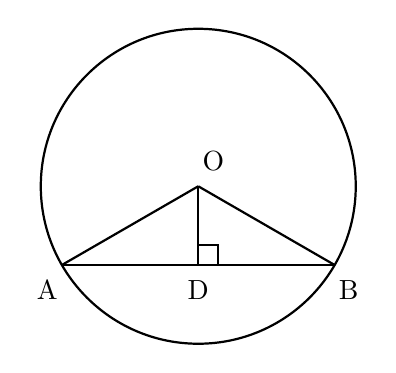
\begin{tikzpicture}[scale=1]

    % Define the center of the circle
    \coordinate (O) at (0,0);

    % Draw the circle (radius = 2 for good proportions)
    \draw[thick] (O) circle (2);

    % Define points A and B on the circle and D on the chord
    % Placing the chord AB at y = -1 gives a visually accurate proportion
    % x^2 + (-1)^2 = 2^2 => x = +/- sqrt(3) ~ +/- 1.732
    \coordinate (A) at (-1.732, -1);
    \coordinate (B) at (1.732, -1);
    \coordinate (D) at (0, -1);

    % Draw the lines and segments forming the triangle and altitude
    \draw[thick] (A) -- (B);
    \draw[thick] (O) -- (A);
    \draw[thick] (O) -- (B);
    \draw[thick] (O) -- (D);

    % Draw the right-angle symbol at D
    \draw[thick] (0.25, -1) -- (0.25, -0.75) -- (0, -0.75);

    % Add labels for the points
    \node[above right, xshift=-2pt, yshift=2pt] at (O) {O};
    \node[below left, xshift=2pt, yshift=-2pt] at (A) {A};
    \node[below right, xshift=-2pt, yshift=-2pt] at (B) {B};
    \node[below, yshift=-2pt] at (D) {D};

\end{tikzpicture}